% !TeX spellcheck = de_DE
%
% Folien getestet mit: latexmk -lualatex --shell-escape -silent -latexoption="-synctex=1" %
% Argumente werden direkt an die Beamer-Class weitergeben
% aspectratio=43 | 169 | 1610 
% Getestet wird mit 1610
% Auf Linux eignet sich https://pdfpc.github.io/ zum präsentieren
%

\documentclass[aspectratio=169,usenames,dvipsnames,rgb]{../tuprolis}
\metroset{subsectionpage=progressbar}
\usetikzlibrary{calc}
\usepackage{tikz}
\usetikzlibrary{backgrounds,calc,positioning}
\usepackage{pgfplots}
\usepackage{listings}
\usepackage{pgfpages}
\usepackage{xparse}
\usepackage[binary-units,per-mode=repeated-symbol]{siunitx}
\sisetup{locale=DE}
\DeclareSIUnit{\packets}{\ensuremath{p}}
\usepackage{standalone}
\usepackage{bytefield}
\usepackage{varwidth}
\usepackage{svg}
\usepackage{adjustbox}

%\setbeameroption{show notes on second screen}
\usetikzlibrary{decorations.pathreplacing,shapes,positioning,arrows,automata,positioning,shapes,fit,plotmarks,decorations,decorations.pathreplacing,arrows,intersections, pgfplots.fillbetween, calc,backgrounds,decorations.markings}
\usepackage[backend=biber]{biblatex}
\addbibresource{../bib/source.bib}
\nocite{*} 

\newcommand{\tikzmark}[1]{\tikz[baseline={(#1.base)},overlay,remember picture] \node[outer sep=0pt, inner sep=0pt] (#1) {\phantom{A}};}

%% syntax
%%%\mybrace{<first>}{<second>}[<Optional text>]
\NewDocumentCommand\mybrace{mmo}{%
	\IfValueTF {#3}{%
		\begin{tikzpicture}[overlay, remember picture,decoration={brace,amplitude=1ex}]
		\draw[decorate,thick] (#1.north east) -- (#2.south east) node[midway, right=0.1cm] {$=$}node[midway, right=0.5cm,text=black,text width = 2in,] {{#3}};
		\end{tikzpicture}%
	}%
	{%
		\begin{tikzpicture}[overlay, remember picture,decoration={brace,amplitude=1ex}]
		\draw[decorate,thick] (#1.north east) -- (#2.south east);
		\end{tikzpicture}%
	}%
}%

\newbibmacro*{author:title:year}{%
	\printnames{labelname}%
	\setunit{\addcolon\space}%
	\printfield[citetitle]{labeltitle}%
	\setunit{\addcomma\space}%
	\printdate
}

\DeclareCiteCommand{\atycite}
{\usebibmacro{prenote}}
{\usebibmacro{author:title:year}}
{\multicitedelim}
{\usebibmacro{postnote}}


\makeatletter
\def\blfootnote{\xdef\@thefnmark{}\@footnotetext}
\makeatother


\usepackage{listings}
\renewcommand\lstlistlistingname{Quellcodeverzeichnis}

\lstset
{ 
	basicstyle=\tiny,
	numbers=left,
	stepnumber=1,
	showstringspaces=false,
	tabsize=1,
	breaklines=true,
	breakatwhitespace=false,
}

\lstdefinelanguage{NED} {
	morekeywords={allowunconnected,bool,channel,channelinterface,connections,const,
		default,double,extends,false,for,gates,if,import,index,inout,input,
		int,like,module,moduleinterface,network,output,package,parameters,
		property,simple,sizeof,string,submodules,this,true,types,volatile,@display
		xml,xmldoc},
	sensitive=true,
	morecomment=[l]{//},
	morestring=[b]",
}

\lstdefinelanguage{INI} {
	morekeywords={},
	sensitive=true,
	morecomment=[l]{\#},
	morestring=[b]",
}

\lstdefinelanguage{ADL} {
	morekeywords={var,retrieve,original,create,change,drop,send,filter,list,from,nodes,do,retrieve,packet,put,destroy},
	sensitive=true,
	morecomment=[l]{\#},
	morestring=[b]",
}


\newcommand{\ned}[1]{\sloppy\texttt{#1}}
\newcommand{\ini}[1]{\sloppy\texttt{\textit{#1}}}
\newcommand{\adl}[1]{\sloppy\textit{\textbf{#1}}}
\newcommand{\csource}[1]{\sloppy\textbf{#1}}
\newcommand{\file}[1]{\sloppy\textit{#1}}

%\setbeameroption{show notes on second screen}
%\setbeameroption{show only notes}

%----------------------------------------------------------
%Beamer Einstellungen
%----------------------------------------------------------

\title{Bachelorabschlussvortrag}

\subtitle{Simulative Analyse von Cyber-Angriffen am Beispiel des Netzes der Fakultät für Informatik der TU Dortmund}

\institute{Bachelorabschlussvortrag am Lehrstuhl 4 - Informatik}

\author{Nils Dunker}

\date{8. Februar 2021}

%----------------------------------------------------------
%Folieninhalt
%----------------------------------------------------------

\usepackage[xindy, toc]{glossaries}
\makeglossaries

\newglossaryentry{seapp}{name={SEA++},description={SEA++ ist ein Netzwerkangriffssimulator für OMNeT++. Er erlaubt die Analyse erfolgreicher Angriffe auf ein Computernetzwerk}}
\newglossaryentry{omnetpp}{name={OMNeT++},description={Ein Discrete-Event-Simulator welcher hauptsächlich für Netzwerksimulationen genutzt wird}}
\newglossaryentry{inet}{name={INET},description={Erweiterung für OMNeT++}}
\newglossaryentry{ned}{name={NED},description={Eine High-Level-Language in der eine (Neztwerk)-Topologie beschrieben werden kann. Steht für Network Description.}}
\newglossaryentry{c++}{name={C++},description={Eine genormte Programmiersprache}}
\newglossaryentry{ethernet}{name={Ethernet},description={Schicht 1 und 2 Übertragungstandard. Standarisiert in IEEE 802.3}}
\newglossaryentry{gnur}{name={GNU R},description={Umgebebung zur Berechnung und Darstellung von Statistiken \cite{GnuRWebsite}}}
\newglossaryentry{python}{name={Python},description={Open Source Porgrammiersprache}}
\newglossaryentry{sterntopologie}{name={Sterntopologie}, plural={Sterntopologien}, description={Eine Sterntopologie verbindet alle Geräte von einem zentralen Knoten aus \cite{Kurose02}}}
\newglossaryentry{git}{name={Git}, description={Eine bekannte verteilte Versionierungssoftware \cite{GitWebsite}}}
\newglossaryentry{svn}{name={SVN}, description={Eine bekannte zentralisierte Versionierungssoftware \cite{SvnWebsite}}}

\newglossaryentry{tcpip}{name={Internet-Protokoll-Stack},description={Der Internet-Protokoll-Stack ist eine Einteilung verschiedner Protokolle in Schichten. Vorgestellt in \autocite{Frystyk1994}. Meist als fünfstelliges Modell wie in \citetitle{Kurose02} \cite{Kurose02} dargestellt}}

\newglossaryentry{layer5}{name={Anwendungsschicht}, description={Oberste Schicht im Internet Protokoll Stack. Die deutsche Bezeichnung ist entnommen aus dem Standardwerk Computernetzwerke \cite{Kurose02}}}
\newglossaryentry{layer4}{name={Transportschicht}, description={Vierte Schicht im Internet Protokoll Stack \cite{Kurose02}}}
\newglossaryentry{layer3}{name={Vermittlungsschicht}, description={Dritte Schicht im Internet Protokoll Stack \cite{Kurose02}}}
\newglossaryentry{layer2}{name={Sicherungsschicht}, description={Zweite Schicht im Internet Protokoll Stack \cite{Kurose02}}}
\newglossaryentry{layer1}{name={Bitübertragungsschicht}, description={Unterste Schicht im Internet Protokoll Stack \cite{Kurose02}}}

\newglossaryentry{ieee8021q}{name={IEEE802.1Q}, description={Standard in dem Grundlagen für VLAN festgeschrieben wurden \cite{8403927}}}

\newglossaryentry{bbbg}{name={BBB},	description={Eine Onlinevideokonferenz Software speziell für die Lehre \cite{BBBWebsite}}}
\newglossaryentry{bbb}{type=\acronymtype, name={BBB}, description={BigBlueButton}, first={BigBlueButton (BBB)\glsadd{bbbg}}, see=[Glossary:]{bbbg}}

\newacronym{igmp}{IGMP}{Internet Group Management Protocol}
\newacronym{icmp}{ICMP}{Internet Control Message Protocol}
\newacronym{ipv4}{IPv4}{Internet Protocol Version 4}
\newacronym{bsi}{BSI}{Bundesamt für Sicherheit in der Informationstechnik}
\newacronym{neta}{NETA}{NETwork Attacks}
\newacronym{ppp}{PPP}{Point-to-Point Protocol}
\newacronym{stp}{STP}{Spanning Tree Protocol}
\newacronym{mitm}{MitM}{Man-in-the-Middle-Angriff}
\newacronym{arp}{ARP}{Address Resolution Protocol}
\newacronym{rfc}{RFC}{Request for Comments}
\newacronym{vss}{VSS}{Virtual Switching System}
\newacronym{vlan}{VLAN}{Virtual Local Area Network}
\newacronym{itmc}{ITMC}{IT \& Medien Centrum}
\newacronym{tu}{TU}{Technische Universität Dortmund}
\newacronym{dnf}{DFN}{Deutsche Forschungsnetz}
\newacronym{irb}{IRB}{Informatikrechner-Betriebsgruppe}
\newacronym{wlan}{WLAN}{Wireless Local Area Network}
\newacronym{adl}{ADL}{Attack Description Language}
\newacronym{asl}{ASL}{Attack Specification Language}
\newacronym{asi}{ASI}{Attack Specification Interpreter}
\newacronym{ase}{ASE}{Attack Specification Engine}
\newacronym{gep}{GEP}{Global Event Processor}
\newacronym{lep}{LEP}{Local Event Processor}
\newacronym{dos}{DoS}{Denial of Service}
\newacronym{dosa}{DoS-Angriff}{Denial-of-Service-Angriff}
\newacronym{ddos}{DDoS}{Distributed Denial of Service}
\newacronym{ddosa}{DDoS}{Distributed-Denial-of-Service-Angriff}
\newacronym{ide}{IDE}{Integrierte Entwicklungsumgebung}
\newacronym{mac}{MAC}{Media Access Control}
\newacronym{csmacd}{CSMA/CD}{Carrier Sense Multiple Access/Collision Detection}
\newacronym{nic}{NIC}{Network Interface Card}
\newacronym{rip}{RIP}{Routing Information Protocol}
\newacronym{bgp}{BGP}{Border Gateway Protocol}
\newacronym{xml}{XML}{Extensible Markup Language}
\newacronym{tcp}{TCP}{Transmission Control Protocol}
\newacronym{udp}{UDP}{User Datagram Protocol}
\newacronym{dsl}{DSL}{domänenspezifische Sprache}
\newacronym{ftp}{FTP}{File Transfer Protocol}
\newacronym{http}{HTTP}{Hypertext Transfer Protocol}
\newacronym{ssh}{SSH}{Secure Shell}
\newacronym{oh}{OH}{Otto-Hahn-Straße}
\newacronym{tucsnet}{Informatiknetzwerk}{Netzwerk der Fakultät Informatik an der TU-Dortmund}
\newacronym{rtt}{RTT}{Round Trip Time}
\newacronym{tls}{TLS}{Transport Layer Security}
\newacronym{pdu}{PDU}{Protocol Data Unit}

\glsaddall

\makeindex

\begin{document}
	
%Deckblatt
\frame[plain]{\titlepage} 

%\begin{frame}[plain]{Inhalt}
%	\tableofcontents[hideallsubsections]
%	\note{
%		Im folgenden werde ich meine Bachelor Arbeit vorstellen. Dabei möchte Ich die wichtigen Komponenten meines Themas vorstellen sowie eine erste Planung meines Vorgehens präsentieren. Zuletzt werde ich kurz auf meine Literatur eingehen .
%		\begin{itemize}
%			\item BA Vorstellen
%			\item Dabei
%			\begin{itemize}
%				\item Thema vorstellen 
%				\item Ablauf
%			\end{itemize}
%		\end{itemize}
%	}
%\end{frame}


\section{Themeneinführung}

\begin{frame}{Thema}
	\begin{block}{Titel}
		Simulative Analyse von Cyber-Angriffen am Beispiel des Netzes der Fakultät für Informatik der TU Dortmund
	\end{block}
	\begin{columns}
		\begin{column}{0.5\textwidth}
			\begin{center}
				Bild aus Urheberrechtsgründen entfernt
			\end{center}
		\end{column}
		\begin{column}{0.5\textwidth}
			\begin{visibleenv}<2>
				\begin{itemize}
					\item Drei Angriffe
					\begin{itemize}
						\item ARP-Spoofing
						\item SYN-Flooding
						\item Port-Scanner
					\end{itemize}
					\item Fokus auf Angriffssimulator
					\item Weitere Einschränkungen
					\begin{itemize}
						\item Nicht Programmieren
						\item Arbeit im direkten Programmökosystem
					\end{itemize}
				\end{itemize}
			\end{visibleenv}
		\end{column}
	\end{columns}
	
	\note{
		\begin{itemize}
			\item Simulative Analyse von Cyber-Angriffen am Beispiel des Netzes der Fakultät für Informatik der TU Dortmund
			\item Titel sehr Allgemein
			\item Deswegen Einschränkungen
			\item Aus ersten Erkenntnissen Fokus auf SEA gelegt
			\item Drei Beispielhafte Angriffe, welche möglichst verschieden sind
			\item Weitere Einschränkungen waren Nötig
			\begin{itemize}
				\item Es werden keine eigenen Module für omnet erstellt und es werden nur dierekte OMNET Programme genutzt. Weitere zu dem Ökosystem kompatible Programme wie Python, R werden nicht betrachtet!
			\end{itemize}
		\end{itemize}
	}
\end{frame}

{
	\metroset{sectionpage=none}
	\section{Werkzeuge}
}

\subsection{OMNeT++, INET und SEA++}
\begin{frame}{OMNeT++ und INET}
	\begin{center}
		\includegraphics[keepaspectratio,
		width=\paperwidth,
		height=0.8\paperheight]{pic/omnet}
	\end{center}

	\note{
		\begin{itemize}
			\item OMNeT++ besteht aus zwei Teilen
			\begin{itemize}
				\item Simulationskern
				\item IDE
			\end{itemize}
			\item Hier Eclipse IDE
			\item Zu sehen INET
			\item Erweiterung für Netzwerkmodule
			\item OMNeT++ und INET in älterer Version wegen SEA++
			\item SEA++ keine IDE
		\end{itemize}
	}
\end{frame} 

\begin{frame}[fragile]{SEA++}
	\includestandalone[width=\textwidth]{tikz/baSeaSystem}
	\begin{onlyenv}<1>
		\begin{center}
			\begin{tabular}{c}
				\lstinputlisting[language=ADL]{listings/example.adl}
			\end{tabular}
		\end{center}
	\end{onlyenv}
	\begin{onlyenv}<2>
		\begin{center}
			\begin{tabular}{c}
				\lstinputlisting[language=XML]{listings/disable.xml}
			\end{tabular}
		\end{center}
	\end{onlyenv}
	\begin{onlyenv}<3>
		\begin{center}
			\includestandalone[keepaspectratio, scale=0.7]{tikz/baSeaGates}
		\end{center}
	\end{onlyenv}

	
	\note{
		\begin{itemize}
			\item SEA besteht aus drei Teilen
			\item Hinweis auf die Probleme durch den Global Filter
			
		\end{itemize}
%		\begin{onlyenv}<1>
%			\begin{itemize}
%				\item SEA++ besteht aus drei Komponenten
%				\item Erste ist die Attack Specification Language oder auch Attack Descritpion Language
%				\item DSL 
%				\item Erlaub Angriffe zu beschreiben
%				\item Definitionen teilweise uneindeutig
%				\item 3 Quellen für die Befehle
%				\begin{itemize}
%					\item Benutzerhandbuch
%					\item Zwei Veröffentlichungen (letzte 2019)
%				\end{itemize}
%				\item Ab hier beginnen die Probleme
%			\end{itemize}
%		\end{onlyenv}
%		\begin{onlyenv}<2>
%			\begin{itemize}
%				\item Interpreter der ADL übersetzt
%				\item Python 2...
%				\begin{itemize}
%					\item[$\Rightarrow$] Fehlende Bibliotheken
%				\end{itemize}
%				\item Befehle werden anders verlangt
%				\begin{itemize}
%					\item Bsp. APP.type muss String sein!
%					\item drop(paket) $\Rightarrow$ drop(paket, schwelle)
%					\item 
%				\end{itemize}
%			\end{itemize}
%		\end{onlyenv}
	}
\end{frame}


\section{Netzwerkmodellierung}
%\begin{frame}[fragile,t]{Vereinfachtes Netzwerk der Informatikfakultät}
%	\begin{columns}[onlytextwidth,t]
%		\begin{column}{0.5\textwidth}
%			\begin{center}
%				\includestandalone[keepaspectratio, scale=0.7]{tikz/baTopReal}
%			\end{center}
%		\end{column}
%		\begin{column}{0.5\textwidth}
%			\begin{center}
%				\textbf{Fakten}
%				\begin{itemize}
%					\item $\sim$ 700 Geräte
%					\item Geringe Auslastung
%					\item Verschiedene Dienste
%					\item \gls{vlan}
%					\item Redundanzen
%				\end{itemize}
%			\end{center}
%		\end{column}
%	\end{columns}
%	\note{
%		Notes
%	}
%\end{frame}

\begin{frame}[fragile]{Netzwerkmodell}
	\vspace{-0.45cm}%
	\begin{center}%
		\begin{adjustbox}{width=\textwidth,height=0.9\textheight, keepaspectratio}
			\includestandalone[]{tikz/baTopKonfig}%
		\end{adjustbox}
	\end{center}%
	\note{
		Notes
	}
\end{frame}

{
	\metroset{sectionpage=none}
	\section{Angriffsmodellierung}
}

\subsection{ARP-Spoofing}
\begin{frame}{ARP-Spoofing Ablauf}
	\begin{columns}
		\begin{column}{0.5\textwidth}
			\begin{center}
				\only<1>{ARP-Anfrage Broadcast}
				\only<2>{ARP-Antwort Unicast}
				\only<3>{ARP-Spoofed-Antwort Unicast}
				\includestandalone[keepaspectratio, width= 0.9\textwidth]{tikz/baArpExample}
			\end{center}
		\end{column}
		\begin{column}{0.5\textwidth}
			\begin{center}
				\begin{onlyenv}<1>
					Anfrage (alice$\Rightarrow$alle)
					\begin{tabular}{|c|c|}
						\hline
						Feld & Wert \\
						\hline
						SHA & 00-00-00-00-00-01 \\
						\hline
						SPA & 1.1.1.1 \\
						\hline
						THA & FF-FF-FF-FF-FF-FF \\
						\hline
						TPA & 1.1.1.2 \\
						\hline
					\end{tabular}
				\end{onlyenv}
				\begin{onlyenv}<2>
					Antwort (bob$\Rightarrow$alice)
					\begin{tabular}{|c|c|}
						\hline
						Feld & Wert \\
						\hline
						SHA & \textcolor{ForestGreen}{00-00-00-00-00-02} \\
						\hline
						SPA & 1.1.1.2 \\
						\hline
						THA & 00-00-00-00-00-01 \\
						\hline
						TPA & 1.1.1.1 \\
						\hline
					\end{tabular}
				\end{onlyenv}
				\begin{onlyenv}<3>
					Antwort (eve$\Rightarrow$alice)
					\begin{tabular}{|c|c|}
						\hline
						Feld & Wert \\
						\hline
						SHA & \textcolor{red}{00-00-00-00-00-03} \\
						\hline
						SPA & 1.1.1.2 \\
						\hline
						THA & 00-00-00-00-00-01 \\
						\hline
						TPA & 1.1.1.1 \\
						\hline
					\end{tabular}
				\end{onlyenv}
				
			\end{center}
		\end{column}
	\end{columns}
	\note{
		Notes
	}
\end{frame}

\begin{frame}[fragile, t]{ARP-Spoofing Umsetzung}
	\begin{onlyenv}<1>
		\begin{block}{Probleme}
			\begin{itemize}
				\item fehlende Hilfsfunktionen
				\item Unterscheidung von Paketfeldern
				\item falsche filter-Implementierung
			\end{itemize}
		\end{block}
		
		\textbf{Datenpakete filtern} \\
		\begin{tabular}{c}
			\lstinputlisting[language=ADL, firstline=0, lastline=4, basicstyle=\scriptsize, firstnumber=1]{listings/arpServer.adl}
		\end{tabular}
	\end{onlyenv}

	\begin{onlyenv}<2>
		\begin{block}{Probleme}
			\begin{itemize}
				\item Vorinitialisierung
			\end{itemize}
		\end{block}
	
		\textbf{Daten auslesen} \\
		\begin{tabular}{c}
			\lstinputlisting[language=ADL, firstline=8, lastline=14, basicstyle=\scriptsize, firstnumber=8]{listings/arpServer.adl}
		\end{tabular}
	\end{onlyenv}


	\begin{onlyenv}<3>
		\begin{block}{Probleme}
			\begin{itemize}
				\item fehlende ARP-Implementierung
			\end{itemize}
		\end{block}
		
		\textbf{Neues ARP-Datenpaket erstellen} \\
		\begin{tabular}{c}
			\lstinputlisting[language=ADL, firstline=16, lastline=26, basicstyle=\scriptsize, firstnumber=16]{listings/arpServer.adl}
		\end{tabular}
	\end{onlyenv}

	\begin{onlyenv}<4>
		\begin{block}{Probleme}
			\begin{itemize}
				\item falsche Dokumentation
			\end{itemize}
		\end{block}
	
		\textbf{Letzte Änderungen} \\
		\begin{tabular}{c}
			\lstinputlisting[language=ADL, firstline=28, lastline=32, basicstyle=\scriptsize,firstnumber=28]{listings/arpServer.adl}
		\end{tabular}
	\end{onlyenv}
	\note{
		Notes
	}
\end{frame}

%\begin{frame}{Probleme bei der Umsetzung}
%	\begin{columns}
%		\begin{column}{0.5\textwidth}
%			\textbf{Fehlende...}
%			\begin{itemize}
%				\item Anbindung der Switches
%				\item ARP-Implementierung
%				\item Hilfsfunktionen
%			\end{itemize}
%		\end{column}
%		\begin{column}{0.5\textwidth}
%			\textbf{Falsche...}
%			\begin{itemize}
%				\item ADL-Definitionen
%				\item Dokumentation
%				\item Implementierung bedingter Angriffe
%			\end{itemize}
%		\end{column}
%	\end{columns}
%\end{frame}

\subsection{SYN-Flooding}

\begin{frame}[fragile]{SYN-Flooding}
	\begin{columns}
		\begin{column}{0.5\textwidth}
			\begin{center}
				\textbf{TCP-Handshake}
				\includestandalone[keepaspectratio]{tikz/baTCPHandshake}
			\end{center}
		\end{column}
		\begin{column}{0.5\textwidth}
			\begin{visibleenv}<1>
				\begin{center}
					\textbf{SYN-Flooding}
					\includestandalone[keepaspectratio]{tikz/baTCPSynFlood}
				\end{center}
			\end{visibleenv}
		\end{column}
	\end{columns}
	
	\note{
		Notes
	}
\end{frame}

\subsection{Firewall-Scanner}

\begin{frame}{ACK-Firewall-Scanner}
%	\visible<1>{\begin{block}{Implementierung}
%Implementierung ähnlich zu den vorherigen Angriff!
%	\end{block}}
	\begin{columns}
		\begin{column}{0.5\textwidth}
			\begin{center}
				\includestandalone[keepaspectratio]{tikz/baTCPAckAnswer}
			\end{center}
		\end{column}
		\begin{column}{0.5\textwidth}
			\begin{center}
				\textbf{Probleme}
				\begin{itemize}
					\item Wissen über Zustand des Systems
					\begin{itemize}
						\item Wurde das Gerät bereits getestet?
					\end{itemize}
					\item Firewall-Module
					\item Port-Range-Definieren
				\end{itemize}
			\end{center}
		\end{column}
	\end{columns}
	
	\note{
		Notes
	}
\end{frame}

%\begin{frame}{SEA++-Änderungen}
%	\begin{columns}[onlytextwidth,t] 
%		\begin{column}{0.5\textwidth}
%			\textbf{Änderungen am Quellcode}
%			\begin{enumerate}
%				\item<1-> Fehlerbehebung
%				\item<2-> Erweiterung um ARP
%				\begin{itemize}
%					\item Erweiterbarkeit beschrieben im Handbuch
%				\end{itemize}
%			\end{enumerate}
%		\end{column}
%		\begin{column}{0.5\textwidth}
%			\begin{onlyenv}<1>
%				\textbf{\adl{filter} $\Rightarrow$ Absturz}
%				\begin{itemize}
%					\item jedes Datenpaket betrachten
%					\item Schicht prüfen 
%					\item wenn Datenpaketklasse unbekannt 
%					\begin{itemize}
%						\item[$\Rightarrow$] Unbehebbarer Fehler
%					\end{itemize}
%				\end{itemize}
%			\end{onlyenv}
%			\begin{onlyenv}<2->
%				\textbf{\only<2>{3}\only<3>{4} Erweiterungen}
%				\begin{enumerate}
%					\item \file{seapputils.cc} $\Rightarrow$ Schicht zurückgeben
%					\item \file{Create.h} $\Rightarrow$ Neues Enum
%					\item \file{Create.cc} $\Rightarrow$ Paket zusammenbauen
%					\item<3> \file{Change.cc} $\Rightarrow$ Typecast
%				\end{enumerate}
%			\end{onlyenv}
%		\end{column}
%	\end{columns}
%\end{frame}


\section{Ergebnisse}

\begin{frame}{Messpunkt}
	\begin{center}
		\includestandalone[keepaspectratio,scale=0.7]{tikz/baTopAngriffArp}
	\end{center}
	\note{
		Notes
	}
\end{frame}


\begin{frame}{ARP-Spoofing}
	\begin{center}
		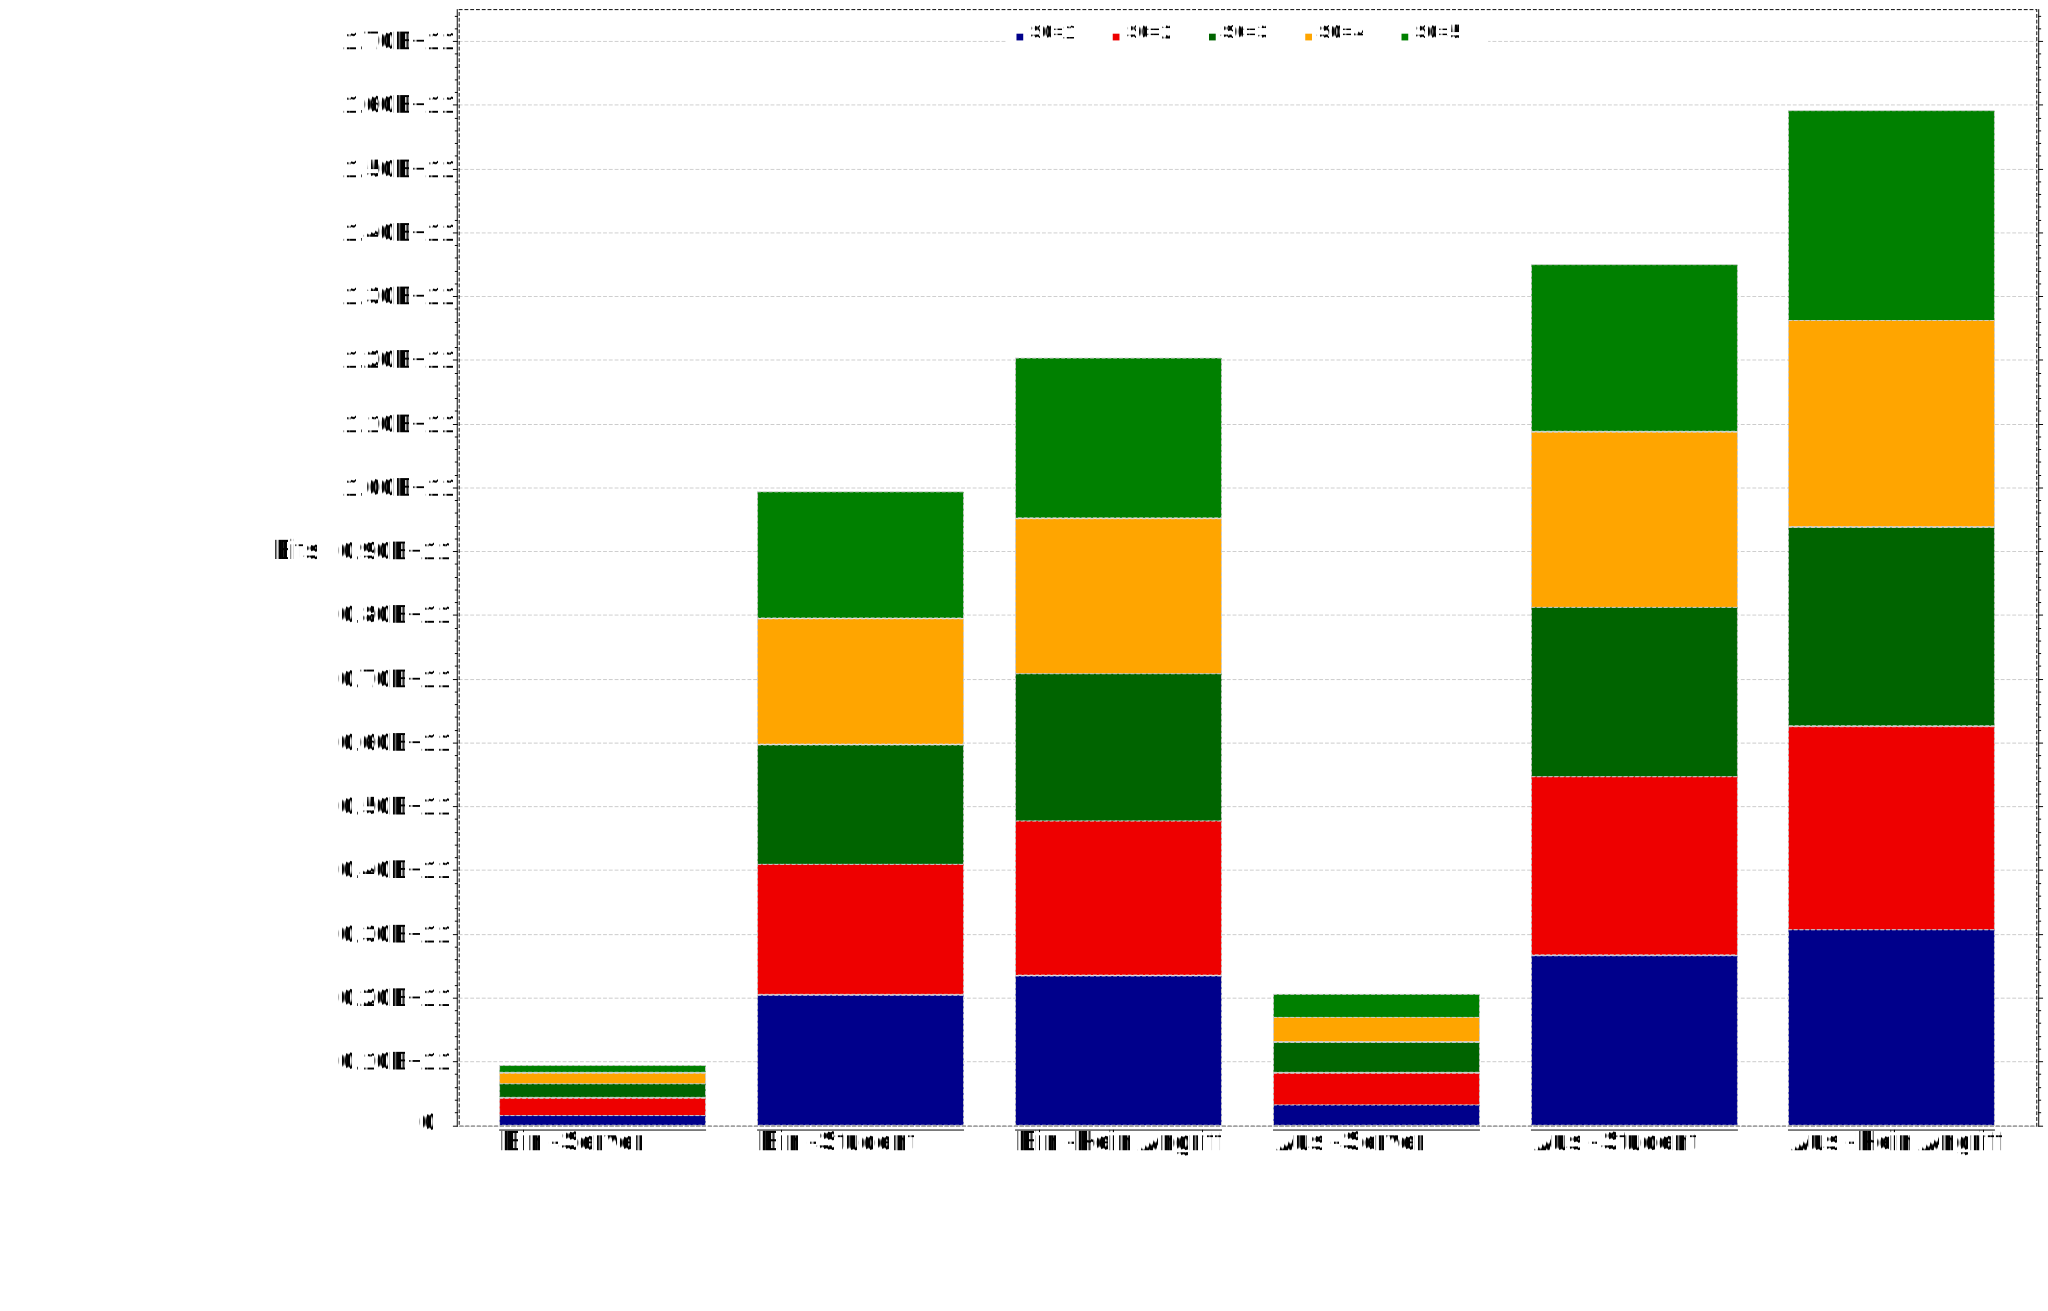
\includegraphics[keepaspectratio,
		width=\paperwidth,
		height=0.8\paperheight]{pic/arp/ArpBitIrb.png}
	\end{center}
	\note{
		Notes
	}
\end{frame}

\begin{frame}{SYN-Flooding}
	\begin{center}
		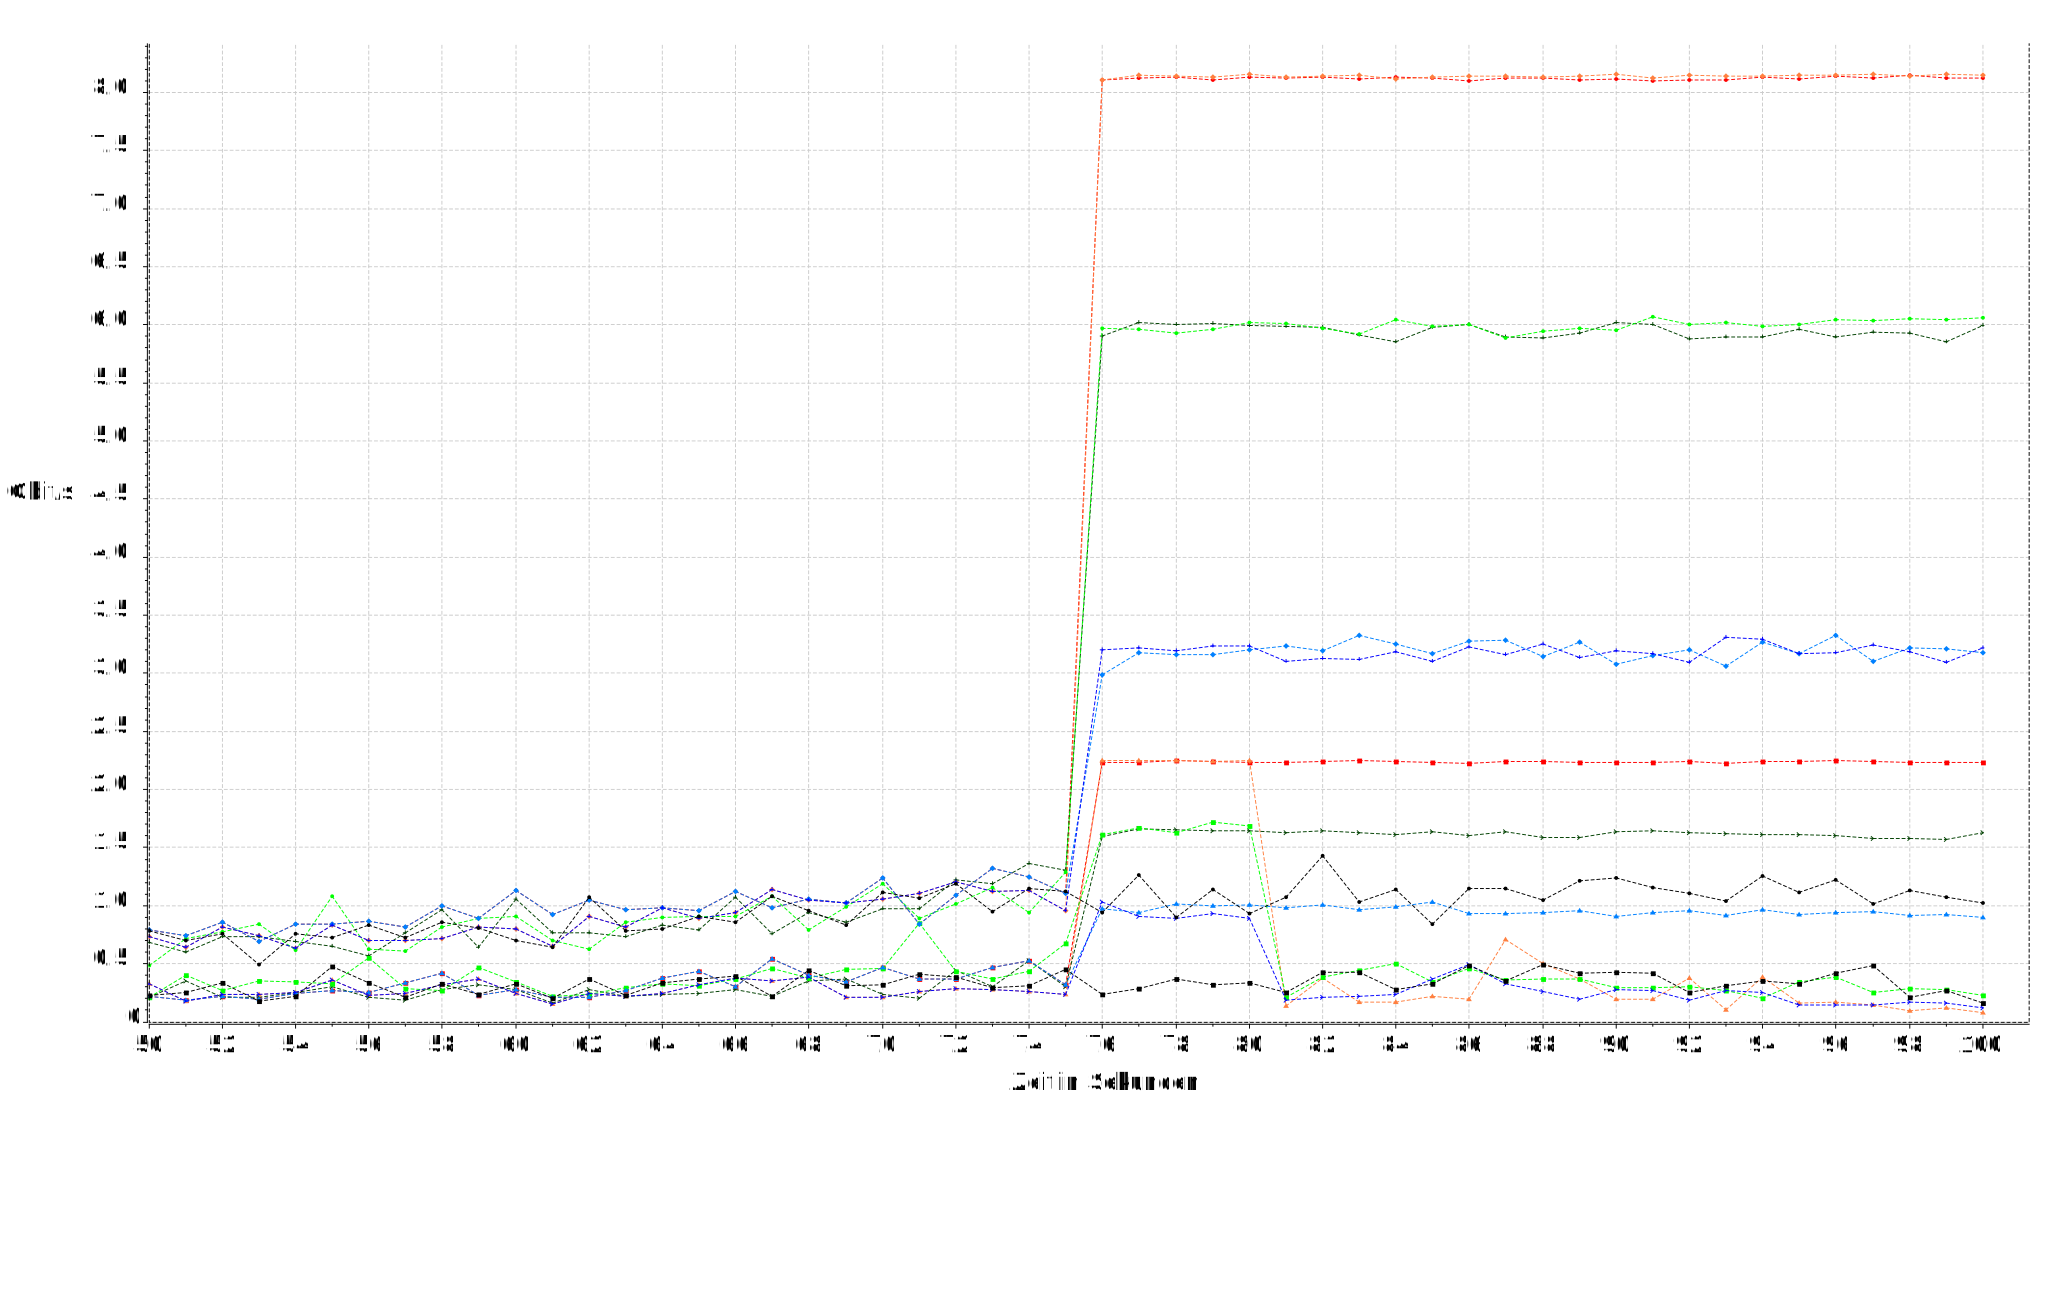
\includegraphics[keepaspectratio,
		width=\paperwidth,
		height=0.8\paperheight]{pic/dos/InternetRouterThruput}
	\end{center}
	\note{
		Notes
	}
\end{frame}

\begin{frame}{Messpunkt}
	\begin{center}
		
		\includestandalone[keepaspectratio,scale=0.7]{tikz/baTopAngriffPort}
	\end{center}
	\note{
		Notes
	}
\end{frame}

\begin{frame}{Firewall-Scanner}
	\begin{center}
		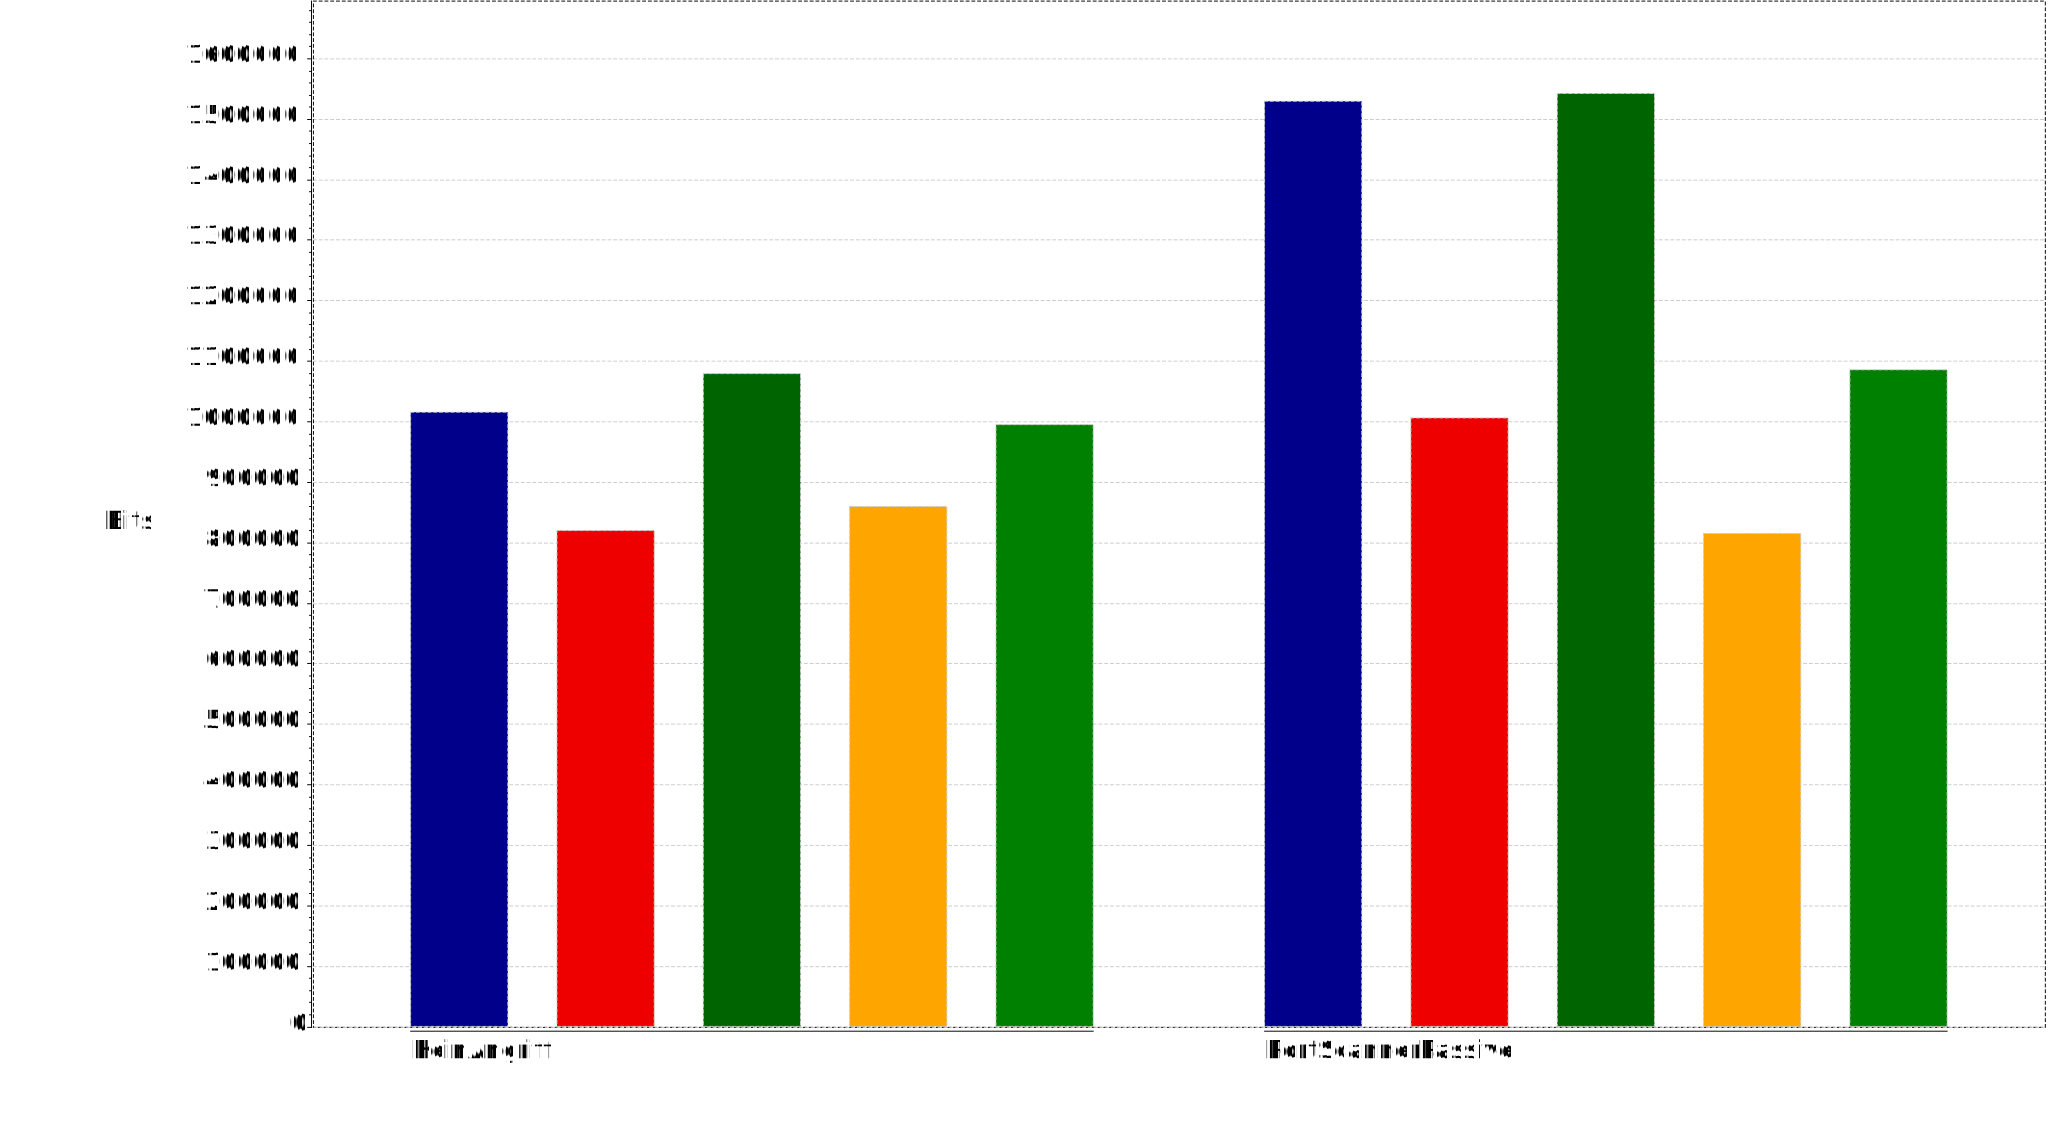
\includegraphics[keepaspectratio,
		width=\paperwidth, 
		height=0.8\paperheight]{pic/port/PortAngriffThruput.png}
	\end{center}
	\note{
		Notes
	}
\end{frame}

\begin{frame}{Zufall in OMNeT++}
	\begin{columns}[] 
		\begin{column}{0.5 \textwidth}
			\textbf{Implementierung des Zufalls}
			\begin{itemize}
				\item Jede Konfiguration besitzt ein Seed
				\item Seed kann festgelegt werden
				\item Zufallsgenerator erzeugt Sequenz aus Zahlen
				\begin{itemize}
					\item[$\Rightarrow$] Immer gleiche Reihenfolge
				\end{itemize}
			\end{itemize}
		\end{column}%
		\begin{column}{0.5 \textwidth}
			\begin{tiny}
				\begin{center}
					\includesvg[width=\textwidth]{pic/zufallTestKlein.svg}
				\end{center}
			\end{tiny}
		\end{column}
	\end{columns}
	\note{
		Notes
	}
\end{frame}


\section{Zusammenfassung}

\begin{frame}{Einordnung der Probleme}
	\begin{columns}[onlytextwidth,t] 
		\begin{column}{0.333 \textwidth}
			\textbf{Primäre}
			\begin{itemize}
				\item Zufallszahlen
				\item Dokumentation
			\end{itemize}
		\end{column}%
		\begin{column}{0.333 \textwidth}
			\textbf{Sekundäre}
			\begin{itemize}
				\item Flexibilität
				\item Modularität
				\item Erweiterbarkeit
				\item ADL-Umfang
			\end{itemize}
		\end{column}
		\begin{column}{0.333 \textwidth}
			\textbf{Weitere}
			\begin{itemize}
				\item Veraltete Basis
				\item Analysetools
				\item Fehlende Module
			\end{itemize}
		\end{column}
	\end{columns}
	\note{
		Notes
	}
\end{frame}

%\begin{frame}{Aussicht}
%	\begin{itemize}
%		\item OMNeT 6.0 
%		\begin{itemize}
%			\item Stark verbessert Analyseumgebung
%			\item neuere IDE
%			\item Wahrscheinlich kompatible zu Ergebnisdateien
%		\end{itemize}
%		\item Wenige Änderungen an SEA++ führen zu großen Verbesserungen
%		\begin{itemize}
%			\item Dokumentation und Versionierung
%			\item Update auf neue Version
%			\item Plugin-System
%		\end{itemize}
%		\item Einige Probleme aufgrund Festlegungen
%		\begin{itemize}
%			\item Analyse mit Python/R besser
%		\end{itemize}
%	\end{itemize}
%	\note{
%		Notes
%	}
%\end{frame}

\begin{frame}{Aussicht}%	
	\begin{center}%
		\begin{adjustbox}{width=\textwidth, height= 0.8\textheight, keepaspectratio}%
			\includegraphics{pic/omnet6}%
		\end{adjustbox}
	\end{center}
	\note{
		Notes
	}
\end{frame}

\appendix
\begin{frame}[allowframebreaks]{Literatur}
    \printbibliography[heading=none]
\end{frame}

\end{document}
